\documentclass{ieeeaccess}
% \RequirePackage{tikz}
% \documentclass[journal]{IEEEtran}
\usepackage{amsmath,amssymb,amsfonts}
\usepackage{physics}
\usepackage{algorithmic}
\usepackage{cite}
\usepackage{graphicx}
\usepackage{textcomp}
\def\BibTeX{{\rm B\kern-.05em{\sc i\kern-.025em b}\kern-.08em
    T\kern-.1667em\lower.7ex\hbox{E}\kern-.125emX}}

% \usepackage{pgfplots}
% \usepackage{standalone}
\usepackage{caption}
% \usepackage{tikz}
% \tikzset{
%   font={\fontsize{10pt}{10}\selectfont}}
%   \usepackage{tikzscale} % Scale the figure not the font
% \usepackage[americanresistors,americaninductors]{circuitikz}
% \usepackage{tikz-dimline} % For dimensional drawing
% \usetikzlibrary{positioning}
% \usetikzlibrary{arrows}
% \usetikzlibrary{patterns}
% \usepackage{subfig}

\usepackage{siunitx} % All the SI unit nomenclature
  \sisetup{per=slash, load=abbr, output-complex-root = j, complex-root-position = before-number, round-mode=figures,round-precision=4}

% Personal definitions
\renewcommand{\v}[1]{\mathbf{#1}} % vectors
\newcommand{\ti}[1]{\tilde{#1}} % spectral representation
\newcommand{\tnsr}[1]{\underline{\underline{#1}}}
% Operators
\renewcommand{\O}{\omega}  % omega
\newcommand{\E}{\varepsilon}  % epsilon
\renewcommand{\u}{\mu}  % mu
\newcommand{\p}{\rho}  % rho
\newcommand{\vp}{\boldsymbol \p}  % rho
\newcommand{\x}{\times}  % times
\renewcommand{\inf}{\infty}  % infinity
\newcommand{\infint}{\int\limits_{-\inf}^\inf} % integral by 
\renewcommand{\del}{\nabla}  % nabla operator
\renewcommand{\^}{\hat}  % unit vector
\newcommand*\diff{\mathop{}\!\mathrm{d}} % Define differential operator
\newcommand{\e}{\mathrm{e}} % Straight-up exponential
\renewcommand{\j}{{j}\mkern1mu} % Straight-up exponential
\newcommand{\iu}{\mathrm{i}\mkern1mu}


\begin{document}
\history{Date of publication xxxx 00, 0000, date of current version xxxx 00, 0000.}
\doi{10.1109/ACCESS.2017.DOI}

\title{Electromagnetic Scattering of Two-dimensional Electromagnetic Systems}
\author{\uppercase{Hasan T. Abbas}\authorrefmark{1,2}, \IEEEmembership{Member, IEEE},
\uppercase{Lilia N. Aljihmani}\authorrefmark{2},
\uppercase{Robert D. Nevels}\authorrefmark{3},\IEEEmembership{Life Fellow, IEEE}
and Khalid A. Qaraqe,
\authorrefmark{2},
\IEEEmembership{Senior Member, IEEE}}
\address[1]{James Watt School of Engineering, University of Glasgow, G12 8QQ UK (e-mail: Hasan.Abbas@glasgow.ac.uk)}
\address[2]{Department of Electrical \& Computer Engineering, Texas A\&M University at Qatar, Doha, 
23874}
\address[3]{Department of Electrical \& Computer Engineering, Texas A\&M University, College Station, TX 77843}
\tfootnote{}

\markboth
{Author \headeretal: Preparation of Papers for IEEE TRANSACTIONS and JOURNALS}
{Author \headeretal: Preparation of Papers for IEEE TRANSACTIONS and JOURNALS}

\corresp{Corresponding author: Hasan T. Abbas (e-mail: Hasan.Abbas@glasgow.ac.uk).}

\begin{abstract}
In this paper, we use the surface equivalence theorem and boundary conditions to develop integral equations to study the electromagnetic (EM) scattering. The proposed scheme is well-suited for investigation of two-dimensional (2D) materials through which engineering of terahertz frequency devices is getting attention. The electronic properties of 2D materials are also discussed with a focus on the existence of plasmons at THz frequencies. Finally, far-field EM scattering response for infinitesimally thin 2D materials is shown at THz frequencies
\end{abstract}

\begin{keywords}
Two-dimensional materials, electromagnetic scattering, terahertz, thin sheets, boundary conditions.
\end{keywords}

\titlepgskip=-15pt

\maketitle

\section{Introduction}
\label{sec:introduction}
\IEEEPARstart{T}{he} emergence of high-precision nanoscale fabrication techniques has led to an increased interest in low dimensional materials due to the extraordinary wave phenomena observed in the the terahertz (THz) to optical frequency regions. Two-dimensional materials are only a few nanometers thick in which electron motion does not face any resistance in a two-dimensional plane. 

In solid-state devices such as a high-electron mobility transistor (HEMT), plasma waves can be generated through current-driven instabilities \cite{Kempa1991}. This phenomenon has led to some breakthrough achievements in the THz frequency region \cite{Dyer2016,Wu2015,Dyakonov1993,Dyakonov1996,Popov2005,Otsuji2006,Dyakonov2005}. A two-dimensional electron gas (2DEG) is formed at the interface of epitaxially grown semiconductors that acts as a transistor channel. In addition to the unusually high electron mobility, free-electron densities that are comparable to metals are observed without any intentional doping in the channel. With the aid of external electromagnetic radiation, plasma waves can be generated in the electron channel of field-effect transistors, which is only a few atoms thick. This was first observed more than 40 years ago \cite{Stern1967a, Allen1977}. One of the most remarkable features of a 2DEG is that frequency response of plasma waves can tuned through external voltage bias \cite{Fatimy2010, Rabbaa2011}. Plasma waves based systems are increasingly becoming pivotal components to couple energy with nanostructure, and in which the energy can be localized to only a few nanometers.

The electromagnetic (EM) analysis for thin conducting sheets is considered challenging as a highly refined mesh is required to accurately resolve the structural details. Historically, approximation methods are used in this regard with approximate boundary conditions, out of which the Leontovich boundary condition (BC) \cite{Senior1995,Hoppe1995} is most well-known, that relates the tangential electric and magnetic fields on the surface of the object as,
%
\begin{equation}
  \v E_{tan} = Z \, \^{\v{n}} \x \v H,
  \label{eq:LBC}
\end{equation} 
% 
where $Z$ is the surface impedance and $\v{\^{n}}$ is the outward unit vector, normal to the surface. Although, the expression in \eqref{eq:LBC} appears to be fairly simple, its accuracy is governed by the material properties as well as the physical complexity of the object. There have been several studies that modify \eqref{eq:LBC} in order for to work for extremely thin and conductive sheets. In one study \cite{Karlsson}, analysis was shown for zero-thickness structures by introducing a material term in the BC. Resistive boundary conditions were introduced in \cite{senior1979backscattering} in which a two-media EM problem was converted to a single medium scattering problem. Other techniques to study the scattering properties of thin sheets involve Nystrom method, in which the structure is analyzed through a discretization scheme \cite{Olga}. Although Nystrom method based techniques are fast, their accuracy is low especially at low discretization orders. 


In this paper, we formulate the scattering response of an infinitesimally thin flat layer of plasma surrounded by free-space using the surface equivalence theorem. The paper is structured as follows. In Section II we first present the dispersion relation of a 2DEG and discuss the electronic properties. We then introduce the integral equation based formulation. Section III shows the numerical results with other similar techniques. Conclusions are summarized in Section IV. This paper is an extension of the work presented in \cite{abbas2017integral,abbas2018electromagnetic}. 

\section{Theory}
\subsection{Dispersion relation}
% 
In a biased HEMT, a 2DEG acts as a transistor channel is formed at the interface of two semiconductor materials of slightly different band-gap energies. Plasma waves are generated in the channel when the source and drain terminals are driven by a current source. A cavity is formed in the channel owing to wave reflection from the conducting boundaries, therefore setting up a standing wave in the channel.

The wavelength of the plasma waves is much shorter than the free-space wavelength at a particular frequency. This compressed nature is typically described by the dispersion relation. Let us consider a HEMT structure surrounded by free-space, and excited by a $\mathrm{TM}$ polarized plane wave. The dispersion relation is obtained by imposing the transverse resonance condition realized by an equivalent transmission line (TL) circuit \cite{Kastner_1988,Michalski2005}. The 2DEG is modeled as a shunt admittance related to Drude-type surface conductivity \cite{Burke2000},
%
\begin{equation}
  Y_{\sigma} = \sigma_s = \frac{N_s e^2 \tau}{m^{\ast}}\frac{1}{1 + \j \O \tau},
  \label{eq:Y2deg}
\end{equation}
%
where $N_s$ is the surface electron density in the channel, $e$ is the electron charge, $m^{\ast}$ is the effective electron mass in the heterostructure, $\tau$ is the scattering time of electrons, and $\O$ is the angular frequency. The dispersion relation is then written as \cite{Gomez-Diaz2012}:
%
\begin{equation}
  Y^{\uparrow}(z_0) + Y^{\downarrow}(z_0) + Y_{\sigma} = 0.
  \label{eq:dispersion}
\end{equation}
%
Here, $Y^{\uparrow}(z_0)$ and $Y^{\downarrow}(z_0)$ are the up- and down-looking TL admittances from the 2DEG located at $z = 0$, and expressed as:
%
\begin{subequations}
  \begin{align}
    Y^{\uparrow}(z_0) &=  Y_2 \frac{1 - \Gamma^{\uparrow}(z_0)}{1 + \Gamma^{\uparrow}(z_0)},
    \label{eq:Yup} \\
    Y^{\downarrow}(z_0) &=  -\j Y_1 \cot (k_{z1} h).
    \label{eq:Ydown}
  \end{align}
  \label{eq:Y}%
\end{subequations}
%
For each layer, $Y_{i}$ and $k_{zi}$ where $i = 0,1,2$ are the respective TM mode admittance and transverse wavenumber of free-space, barrier and substrate layers respectively given by:
%
\begin{align}
  & Y_i = \frac{\O \E_i \E_0}{k_{zi}}, && k_{zi} = \pm \sqrt{k_0^2 \E_i - k_x^2}
  \label{eq:Yandk}
\end{align}
%
where $\E_i$ is the relative permittivity of $i^{\text{th}}$ layer and $k_x$ is the longitudinal propagation constant of the structure. The upward-looking reflection coefficient $\Gamma^{\uparrow}$ in \eqref{eq:Yup} is expressed in terms of the TM mode admittances:
%
\begin{equation}
  \Gamma^{\uparrow}(z_0) = \frac{Y_1 - Y_0}{Y_0 + Y_1} \e^{-2\j k_{z2}d_1}
  \label{eq:Gamma}
\end{equation}
%

\begin{figure}[t!]
  {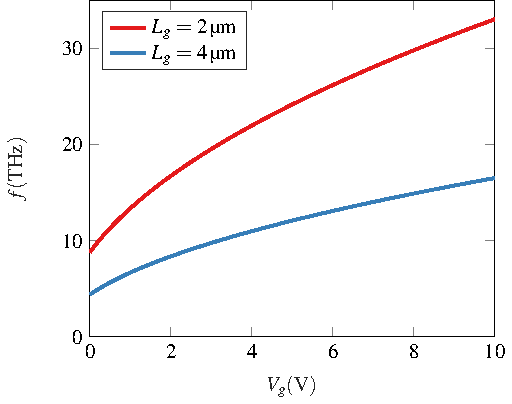
\includegraphics[height=.75\linewidth]{gate_swing.pdf}
  \label{fig:}}
  \caption{Plasma wave Dispersion diagram for the transistor structure supporting a 2DEG channel.}
\end{figure}

% Structure details of GaN/ AlGaN
A closed-form expression for the longitudinal propagation constant $k_x$ by solving \eqref{eq:dispersion} is tedious, therefore numerical root-finding techniques such as the Newton method \cite{9780521880688} have to be employed. As an example, a consider a back-gated transistor consisting of GaN/AlGaN heterostructure, in which the gate-channel separation is $d = \SI{100}{\nm}$. The channel length $L$ is \SI{2}{\micm} whereas the AlGaN barrier layer is $h = \SI{20}{\nm}$ wide.
The permittivity of both semiconductor layers is approximated to the static value, i.e., $\E_1 \approx \E_2 = 9.5$ when the mole-fraction of aluminum in AlGaN alloy is taken as \SI{.2}{} Following \cite{Muravjov2010}, a surface carrier density of $N_s = \SI{5e13}{\cm^{-2}}$ and scattering time $\tau$ of \SI{114}{\ps} corresponding to a temperature of \SI{3}{\kelvin} is assumed. As the temperature is increased, $\tau$ gets smaller which leads to reduced mobility and introduces loss in the channel. $N_s$ can be varied through the gate voltage $V_g$, due to the relation,
%
\begin{equation}
  N_s = N_0 \times \left(1 - \frac{V_g}{V_T} \right),
  \label{eq:tunability}
\end{equation}
%
where $N_0$ is the zero-bias density and $V_T$ is the gate threshold voltage of the transistor. For a channel terminated by highly conducting source and drain terminals at each side, the resonant frequency as a function of carrier density is expressed as \cite{Popov2008}:
%
\begin{equation}
  \O = \sqrt{\frac{N_s \e^2 d}{m_{\ast} \E}} \frac{\pi}{L}
  \label{eq:plasma_frq}
\end{equation}
%
where $\E$ is the average permittivity of the surrounding media. Using \eqref{eq:tunability} and \eqref{eq:plasma_frq}, the tunability of plasma waves assuming a gate threshold voltage of \SI{-.764}{\volt} is shown in Fig. \ref{fig:tuning}. As expected, increasing the length of the channel reduces the resonant frequency.

\begin{figure*}[!t]
% ensure that we have normalsize text
\normalsize
% Store the current equation number.
\setcounter{MYtempeqncnt}{\value{equation}}
% Set the equation number to one less than the one
% desired for the first equation here.
% The value here will have to changed if equations
% are added or removed prior to the place these
% equations are referenced in the main text.
\setcounter{equation}{8}
\begin{equation}
\label{eq:E1scatt}
\v E_1 =
    -\frac{\O}{4 k_1^2} \left( k_1^2 + \del \del \cdot \right) \int\limits_{C} \v J_s(\vp') H_0^{(2)}(k_1 |\vp - \vp'|) \diff{l'}
    - \frac{1}{4 \E \j} \del \x \int\limits_{l} \v M_s(\vp') H_0^{(2)}(k_1 |\vp - \vp'|) \diff{l'} + \v E^i
\end{equation}
\begin{equation}
\label{eq:H1scatt}
    \v H_1 =
    \frac{1}{4 \j} \del \x \int\limits_{l} \v J_s(\vp') H_0^{(2)}(k_1 |\vp - \vp'|) \diff{l'} 
    -\frac{\O}{4 k_1^2} \left( k_1^2 + \del \del \cdot \right) \int\limits_{l} \v M_s(\vp') H_0^{(2)}(k_1 |\vp - \vp'|) \diff{l'} + \v H^i
\end{equation}
\begin{equation}
\label{eq:E2scatt}
    \v E_2 = 
    -\frac{\O}{4 k_2^2} \left( k_2^2 + \del \del \cdot \right) \int\limits_{C} \left(-\v J_s(\vp')\right) H_0^{(2)}(k_2 |\vp - \vp'|) \diff{l'}
    - \frac{1}{4 \j} \del \x \int\limits_{l} \left(-\v M_s(\vp')\right) H_0^{(2)}(k_2 |\vp - \vp'|) \diff{l'}
\end{equation}
\begin{equation}
\label{eq:H2scatt}
    \v H_2 =
    \frac{1}{4 \j} \del \x \int\limits_{l} \left(-\v J_s(\vp')\right) H_0^{(2)}(k_2 |\vp - \vp'|) \diff{l'} 
    -\frac{\O}{4 k_2^2} \left( k_2^2 + \del \del \cdot \right) \int\limits_{l} \left(-\v M_s(\vp')\right) H_0^{(2)}(k_2 |\vp - \vp'|) \diff{l'}
\end{equation}
% Restore the current equation number.
\setcounter{equation}{\value{MYtempeqncnt}}
% The IEEE uses as a separator
\hrulefill
% The spacer can be tweaked to stop underfull vboxes.
\end{figure*}

\subsection{Surface Equivalence Theorem}
%
The field computation due to sources present in an inhomogeneous environment can be simplified using the surface equivalence theorem in which the actual sources are replaced by a set of fictitious, yet equivalent sources. The solution can be divided into two homogeneous spaces, one internal and the other exterior. The total fields in the external region are due to equivalent electric and magnetic surface currents, $\v J_s$ and $\v M_s$ respectively.  In case when the object is collapsed to a flat sheet, the fields can be expressed as in \eqref{eq:E1scatt} and \eqref{eq:H1scatt}, where $\v E^i$ and $\v H^i$ are the incident electric and magnetic fields that are known, $k_1$ is the free-space propagation constant, $\vp$ and $\vp'$ are the position vectors of any point from the origin and source respectively, and $H_0^2(\cdot)$ is the zero order Hankel function of the second kind.  Similarly, fields for the interior region that only contain the scattered part are given in \eqref{eq:E2scatt} and \eqref{eq:H2scatt}, where $k_2$ is the propagation constant in the interior region.
%

\subsection{Surface Integral Equation}
%
\subsubsection{$\mathbf{TM_z}$ Polarization for Plasma-wave Excitation}
%
Next we consider a $\mathrm{TM_z}$ excited planar dielectric sheet lying along the x-axis and apply the surface equivalence theorem to find the electric ($\v J_s$) and magnetic  ($\v M_s$) currents on the sheet,
\setcounter{equation}{12}
\begin{subequations}
  \begin{align}
    \v J_s &=  \hat{\v{n}} \x \v{H} = \hat {\v{z}} \, \mathrm{J(\xi)},
    \label{eq:J_s}\\
    \v M_s &=  -\hat{\v{n}} \x \v{E} = \hat {\v{x}} \, \mathrm{M(\xi)}
    \label{eq:M_s}
  \end{align}
  \label{eq:eq_currents}%
\end{subequations}%
%
where the normal unit vector $\hat{\v{n}}$ is in the y direction and $\xi$ depends on $x$ and $y$ coordinates. Suppose a plane wave propagating along the direction $\v{k}$ with electric field $\v{E}$ polarized along the z direction is incident on the dielectric surface at an angle $\phi_i$. To find the surface currents, we set up an homogeneous equivalent problem first for the region outside the dielectric sheet due to an incident field,
%
\begin{equation}
  \v E^i = \hat{\v z} \; E_0  \e^{-\j k_1 (x \cos \phi_i - y \sin \phi_i)}
  \label{eq:E_i}
\end{equation}
%
with $E_0$ the amplitude of the incoming plane wave. We now express the scattered fields in terms of potentials as
%
\begin{subequations}
  \begin{align}
    \v E_1^{scat} &=  -\frac{\j \O}{k_1^2}\left( k_1^2 + \del \del \cdot \right) \v A,
    \label{eq:E1scat}\\
    \v H_1^{scat} &=  -\frac{\j \O}{k_1^2}\left( k_1^2 + \del \del \cdot \right) \v F,
    \label{eq:H1scat}
  \end{align}
  \label{eq:1scat_pot}%
\end{subequations}%
%
where $\v A$ and $\v F$ are the magnetic and electric vector potentials respectively, given by:
%
\begin{subequations}
  \begin{align}
    \v A &=  \frac{\u}{4 \j} \int\limits_{l} \v J_s(\vp') H_0^{(2)}(k_1 |\vp - \vp'|) \diff{l'},
    \label{eq:A}\\
    \v F &=  \frac{\E}{4 \j} \int\limits_{l} \v M_s(\vp') H_0^{(2)}(k_1 |\vp - \vp'|) \diff{l'},
    \label{eq:Fig}
  \end{align}
  \label{eq:potentials_2d}%
\end{subequations}%
%
The scattered electric field off a flat plate oriented along the x-axis can be simply written in a scalar form due to a $z$-directed incident wave,
%
\begin{equation}
  \begin{split}
    E_1^{scat} &= -\j \O \mathrm A_z \\
    &= - \frac{\O \u}{4 j} \int\limits_{l} J_z(x')  H_0^{(2)}(k_1 |\vp - \vp'|) \diff{l'}
    \label{eq:E1sc_scalar}
  \end{split}
\end{equation}
%
% Likewise, the magnetic field that is tangential to the plate is,
% %
% \begin{figure*}[!t]
% % ensure that we have normalsize text
% \normalsize
% % Store the current equation number.
% \setcounter{MYtempeqncnt}{\value{equation}}
% % Set the equation number to one less than the one
% % desired for the first equation here.
% % The value here will have to changed if equations
% % are added or removed prior to the place these
% % equations are referenced in the main text.
% \setcounter{equation}{17}
% \begin{equation}
%   \begin{split}
%     H_{1,x}^{scat} = 
%      -\frac{\j \O}{k_1^2}\left(k_1^2 +  \pdv[2]{}{x} \right) \int\limits_{l} M_x(x') H_0^{(2)}(k_1 |x - x'|) \diff{l'}.
%   \end{split}
%   \label{eq:H1sc_scalar}
% \end{equation}
% % Restore the current equation number.
% % The IEEE uses as a separator
% \hrulefill
% % The spacer can be tweaked to stop underfull vboxes.
% \end{figure*}
% \begin{equation*}
%   \begin{split}
%     H_{1,x}^{scat} &= -\frac{\j \O}{k_1^2}\left(k_0^2 +  \pdv[2]{}{x} \right) \mathrm F_x \\
%     &= -\frac{\j \O}{k_1^2}\left(k_1^2 +  \pdv[2]{}{x} \right) \int\limits_{l} M_x(x') H_0^{(2)}(k_1 |x - x'|) \diff{l'}.
%   \end{split}
%   \label{eq:H1sc_scalar}
% \end{equation*}
%
Using a similar procedure, we set up an interior equivalent with the currents reversing the signs. The total fields for the interior region only contain the scattered fields.
%
\begin{subequations}
  \begin{align}
    E_2^{scat} &= -\frac{\O \u}{4 \j} \int\limits_{l} -J_z(x')  H_0^{(2)}(k_2 |x - x'|) \diff{l'}
    \label{eq:E2sc}\\
    H_{2,x}^{scat} &= - \frac{\j \O}{k_2^2}\left(k_2^2 +  \pdv[2]{}{x} \right) \nonumber \\  & \int\limits_{l} -M_x(x') H_0^{(2)}(k_2 |x - x'|) \diff{l'}.
    \label{eq:H2sc}
  \end{align}
  \label{eq:2sc}%
\end{subequations}%
% 
In order to find the electric and magnetic currents, we apply the boundary conditions at the interface ensuring the continuity of tangential component of the fields. At the interface:
%
\begin{subequations}
  \begin{align}
    \^{\v n} \x (\v E_1 - \v E_2) ={}& \v 0
    \label{eq:BC_E}\\
    \^{\v n} \x (\v H_1 - \v H_2) ={}& \v 0
    \label{eq:BC_H}
  \end{align}
  \label{eq:BC}%
\end{subequations}%
%
\begin{figure}[!t]
  \centering
  {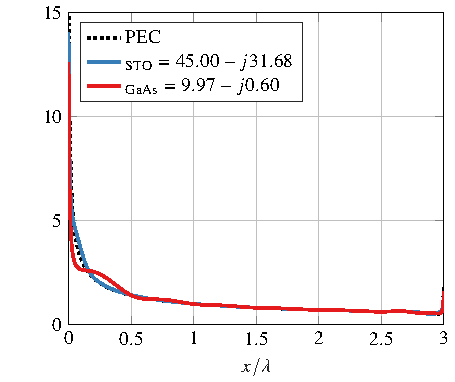
\includegraphics[width=3in]{current_edgeon_3.pdf}
      }
  \caption{Current Distributions on a $3\lambda$ plate at edge-on incidence for PEC, strontium titanate (STO) and gallium arsenide (GaAs).}
  \label{fig:edgeon}
\end{figure}
% 
Using \eqref{eq:BC_E}, \eqref{eq:E1sc_scalar} and \eqref{eq:H2sc} we obtain:
%
\begin{align}
  E_i &= \frac{\O \u}{4} \int\limits_c J_z(x') \left[ H_0^{(2)}(k_1 X) + H_0^{(2)}(k_2 X)\right] \diff{l'},
  \label{eq:scalarE}
\end{align}
where the superscript $tan$ indicates the tangential component of the incident magnetic field in the x-direction. Equation 9 represents an integro-differential equation in which the differential and integral operators on the right hand side may be interchanged. Operators with the order as in \eqref{eq:scalarH_pock} represent \emph{Pocklington's} integro-differential equation \cite{Stutzman2012}. The second order derivative can be removed by expressing in terms of other Hankel functions through the recurrence relations \cite[p. 361]{Abramowitz2012}.
%
\begin{subequations}
  \begin{align}
    \dv{H_0^{(2)}(x)}{x} &= -H_{1}^{(2)}(x) + \frac{1}{x} H_0^{(2)}(x)
    \label{eq:Hankel_ID1}\\
    H_{1}^{(2)}(x)  &= \frac{x}{2} \left[H_{0}^{(2)}(x) + H_{2}^{(2)}(x)\right]
    \label{eq:Hankel_ID2}
  \end{align}
  \label{eq:Hankel_ID}%
\end{subequations}%
%
\section{Numerical Results}
%
A method of moments (MoM) solution to compute the currents is implemented using pulse basis functions with point matching method \cite{Harrington1993} that converts the integral equations into a linear system of equations,
%
\begin{equation}
\begin{bmatrix}
  Z_{mn}   & 0 \\
  0        & Y_{mn}
\end{bmatrix}
\begin{bmatrix}
  J_n \\
  M_n
\end{bmatrix}
=
\begin{bmatrix}
  E_m^i \\
  H_m^i
\end{bmatrix}
\label{eq:MOM}
\end{equation}
%
where $Z_mn$ and $Y_mn$ are the impedance and admittance terms respectively.

\subsection{Current Distribution}
%
Figure. \ref{fig:edgeon} shows the absolute value of the tangential surface electric current on a $\mathrm{TM_z}$ polarized plate of length $3 \lambda$ at edge-on ($\phi_i = \pi$). The discontinuity seen at the edge is a typical behaviour commonly known as wedge condition, which is responsible for EM radiation. Gallium Arsenide ($\mathrm{GaAs}$) and Strontium Titanate ($\mathrm{SrTiO_3}$) sheets are considered at terahertz frequencies where material data has been taken from measurements in \cite{burke2000} and \cite{herranz2012high} respectively, and the results are compared with a perfect electric conductor (PEC) plate of same length \cite{senior1979backscattering}. It is noted that the material having a lower dielectric constant produces less sharp discontinuity at the edge where the wave is incident.
%
\begin{figure}[!t]
  \centering
  \subfloat{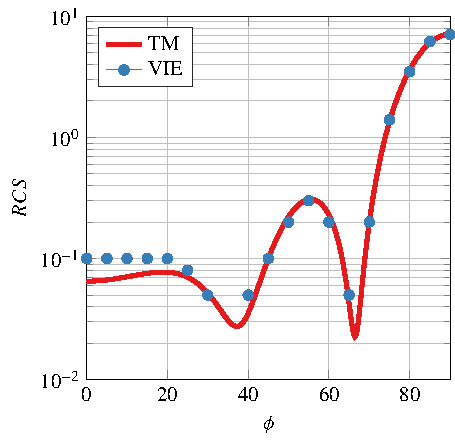
\includegraphics[width=2.85in]{richmond_tm.pdf}
  \label{fig:TM_rcs}} 
  \subfloat{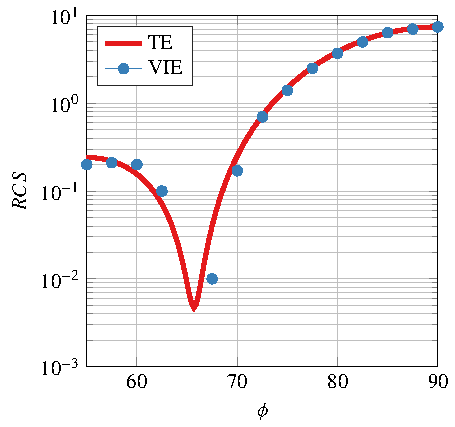
\includegraphics[width=3in]{richmond_te.pdf}
  \label{fig:TE_rcs}}
  \caption{Computed RCS of a $2.5 \lambda$ dielectric rod of permittivity $\E=4$ (a) $\mathrm{TM_z}$, (b) $\mathrm{TE_z}$}
  \label{fig:RCS_richmodn}
\end{figure}
%
\subsection{Far-field}
%
The scattered electric field in the far-zone can be expressed by normalizing the large argument approximation of Hankel functions as:
%
\begin{equation}
  \lim_{k_1|\vp - \vp'|\to\inf} E_z(\vp) \simeq \int \limits_{0}^{L} J_z(x') \e^{\j k_1 x' \cos(\phi_i)} \diff{x'}
  \label{eq:far-field}
\end{equation}
%
where $\phi_i$ is the angle of incidence. The results of our scheme are compared with other techniques that have been used in the context of thin sheets. First, the far-field patterns of $\mathrm{TM_z}$ polarized dielectric sheet of permittivity $\E = 4$ are compared with results in \cite{Richmond1965}, which was the first to apply an integral equation technique to simulate thin structures ans uses a volume integral equation (VIE) technique, which is then collapsed to the surface of the structure. The length of the dielectric sheet is taken as $2.5 \lambda$ and the radar cross-sections (RCS) are shown in Fig. \ref{fig:RCS_richmodn}. The disparity near edge-on condition is due to the fact that the structure considered in \cite{Richmond1965} had a thickness of $0.05 \lambda$, whereas in this work, we have taken an infinitesimally thin sheet. Through  similar steps, the $\mathrm{TE_z}$ scattering expression can be obtained and the results are shown in Fig. \ref{fig:RCS_richmodn}b. The difference in the absorption observed is again attributed to the dissimilar thicknesses of the two structures.
% 

%
%
%
%
\section{Conclusion}
We present a new class of surface integral equations for infinitesimally thin dielectric sheets based on the surface equivalence theorem. The proposed method is well-suited to study the scattering properties of extremely thin structures such as two-dimensional materials, that are increasing become significant thanks to their capability to couple radiation with nanostructures, especially in the terahertz frequency range.

% \section*{Acknowledgment}

% The preferred spelling of the word ``acknowledgment'' in American English is 
% without an ``e'' after the ``g.'' Use the singular heading even if you have 
% many acknowledgments. Avoid expressions such as ``One of us (S.B.A.) would 
% like to thank $\ldots$ .'' Instead, write ``F. A. Author thanks $\ldots$ .'' In most 
% cases, sponsor and financial support acknowledgments are placed in the 
% unnumbered footnote on the first page, not here.

% \section*{References}

\bibliography{Combined}
\bibliographystyle{IEEEtran}

\EOD

\end{document}

